\section{Introduction}
\label{sec:introduction}

The increasing availability of big data and machine learning techniques brings out the importance of data in modern software systems.
Data become a cornerstone piece to autonomously derive decisions from them, or at least to support decision-making processes.
This trend has also been recognized by official institutions, like Datalandscape\footnote{\url{http://datalandscape.eu}}, a European institution analyzing the so-called \textit{data market}.
A recent example is Industry 4.0~\cite{DBLP:journals/bise/LasiFKFH14}, where factories are increasingly automated by analyzing data coming from different sensors and controlling processes based on this.

However, \textbf{data are inherently uncertain}. 
Data collected from sensors contain the uncertainty due to their accuracy and failure rate~\cite{DBLP:conf/asplos/BornholtMM14, metrology2008evaluation} or malicious false data injection~\cite{liang20172015}.
Uncertainty can also be the result of human errors when entering data in a system.
Also, simulation or forecast techniques carry uncertainty in their results.
The same counts for all machine learning algorithms.

A software system \textbf{not considering this uncertainty would lead to a potentially catastrophic situation}, as a misperception of the reality of the system may lead to wrong decisions~\cite{DBLP:conf/asplos/BornholtMM14}.
Uncertainty blurs the human's or algorithm's understanding of a situation or system state.
James Bornholt shows in~\cite{bornholt2013abstractions} that computing the average speed during a walking activity and ignoring the uncertainty of GPS data lead to unrealistic situations such a walking speed equals to 95 km/h.
Another example in the smart grid domain is the load approximation.
Ignoring the uncertainty of the grid topology may lead to a false detection of an overloading incident.\looseness-1

On the one hand, developers ignore this uncertainty.
As shown by James Bornholt~\cite{bornholt2013abstractions}, over 100 popular applications which use GPS location, only one considers the uncertainty of data manipulated.
On the other hand, scientific computing software devotes a significant portion of their code to the management of uncertainty.
This claim is supported by the existence of frameworks such as the GUM~\cite{metrology2008evaluation}, made by the Joint Committee for Guides in Metrology\footnote{\url{https://www.bipm.org/en/committees/jc/jcgm/}}, or OpenTurns~\cite{baudin2017openturns}, a framework supported by companies expert or using scientific computing.

\textbf{Developing such software systems requires significant expertise in handling uncertainty (probability and statistics theory)} to efficiently manipulate and interpret data. 
Several techniques based on probability theory and fuzzy logic have been proposed~\cite{zadeh1996fuzzy,metrology2008evaluation,shafer1992dempster} to handle uncertainty. 
The application of these techniques requires a deep understanding of the underlying theories and is a time-consuming task~\cite{DBLP:conf/quatic/VallecilloMO16}.
Moreover, it is hard to test and, perhaps most importantly, very error-prone.

Different works implement the theory behind uncertainty management in the form of libraries or frameworks~\cite{url:InferNET18, baudin2017openturns}.  
In this chapter, we argue that using a library or a framework to handle uncertainty is efficient in terms of reusability but it fails to prevent the most common errors during development time. 
For example, all errors and bugs related to type inconsistencies and mismatches (semantics error) will be discovered only at runtime.
As done by Vallecillo~\etal in~\cite{DBLP:conf/quatic/VallecilloMO16}, we argue that \textbf{an efficient solution to handle data uncertainty in software systems should be realized at the language level itself with a first-class citizen}. 
Having it on the language level enhances library and framework-based approaches by adding a static, uncertainty-aware type system which is able to detect type errors at development time.\looseness-1

In this chapter, we describe the following contributions: 
\begin{itemize}
	\vspace{-0.5em}
	\setlength\itemsep{-0.3em}
    \item Description and definition of the main concepts and operators to introduce in a language with uncertainty as a first-class citizen. Doing so, developers will be able to manipulate uncertain and certain data in a similar way, hiding complex concepts behind ones they are used to. 
    \item An uncertainty-aware static type checker enabling the design-time detection of programming errors. This type checker can be used as \textit{implicit documentation}, which helps developers in implementing uncertainty-aware algorithms.
    \item We implement these two contributions in the \langName{} language, publicly available\footnote{\url{https://github.com/lmouline/aintea/}}. An overview of this language is depicted in \autoref{fig:motivation-aintea-overview}. Then, we use a real-world case study, built with our partner Creos S.A., to answer the two following research questions: 
    \begin{itemize}
   		\vspace{-0.5em}
		\setlength\itemsep{-0.3em}
    	\item \textit{RQ1:} Does the uncertainty management have an impact on the conciseness of a language? 
		\item \textit{RQ2:} Can the type system detect errors related to uncertainty management?
    \end{itemize}
\end{itemize}

Our use-case implementation shows first that our approach does not impact the conciseness of the language (RQ1).
Second, it highlights the feasibility and the advantages (RQ2) of an uncertainty-aware type checking system on the language level.

The remainder of this chapter is as follows.
In \Cref{sec:aintea:duc}, we present and discuss the main concepts and operators for uncertainty management as a first-class citizen of a language. 
\Cref{sec:aintea:validation} presents our \langName{} implementation and validates the design time error detection and its impact on language conciseness. 
\Cref{sec:aintea:conclusion} concludes and presents some open research perspectives. 


\begin{figure}
	\centering
	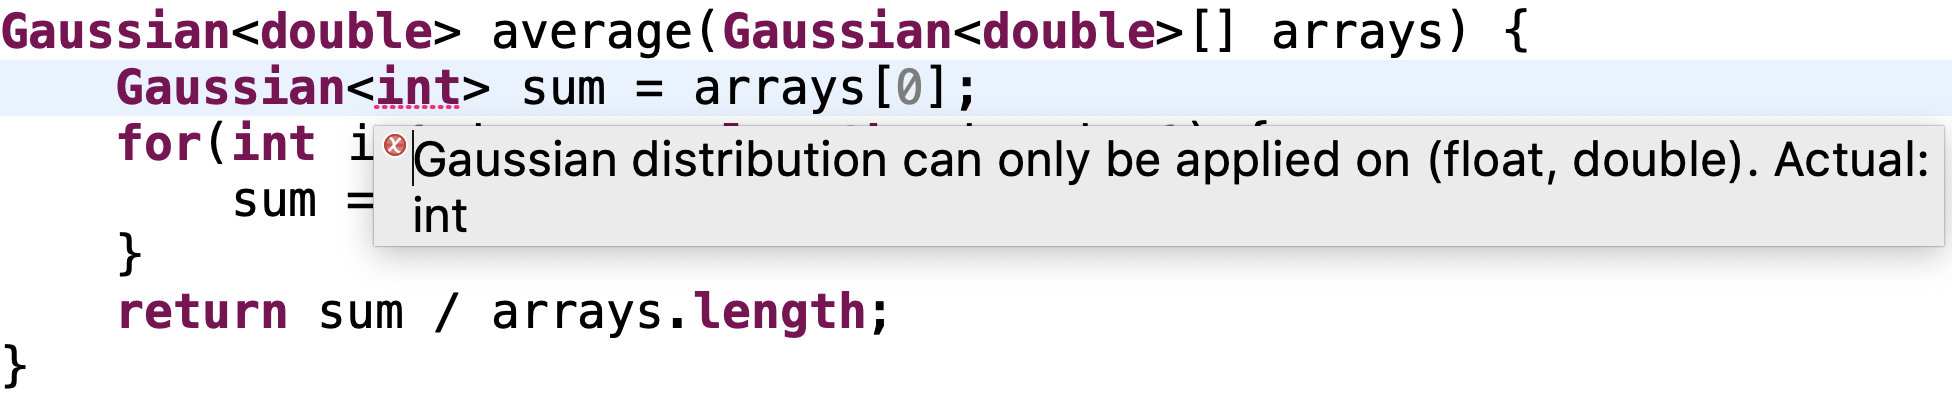
\includegraphics[width=\linewidth]{img/chapt-aintea/intro/aintea-overview}
	\caption{Overview of the language proposed, \langName{}}
	\label{fig:motivation-aintea-overview}
\end{figure}